\documentclass[12pt]{report}
\usepackage[utf8]{inputenc}
\usepackage[russian]{babel}
%\usepackage[14pt]{extsizes}
\usepackage{listings}
\usepackage{graphicx}
\usepackage{amsmath,amsfonts,amssymb,amsthm,mathtools} 
\usepackage{pgfplots}
\usepackage{filecontents}
\usepackage{indentfirst}
\usepackage{eucal}
\usepackage{amsmath}
\usepackage{enumitem}
\frenchspacing

\usepackage{indentfirst} % Красная строка


%\usetikzlibrary{datavisualization}
%\usetikzlibrary{datavisualization.formats.functions}

\usepackage{amsmath}




% Для листинга кода:
\lstset{ %
language=haskell,                 % выбор языка для подсветки (здесь это С)
basicstyle=\small\sffamily, % размер и начертание шрифта для подсветки кода
numbers=left,               % где поставить нумерацию строк (слева\справа)
numberstyle=\tiny,           % размер шрифта для номеров строк
stepnumber=1,                   % размер шага между двумя номерами строк
numbersep=5pt,                % как далеко отстоят номера строк от подсвечиваемого кода
showspaces=false,            % показывать или нет пробелы специальными отступами
showstringspaces=false,      % показывать или нет пробелы в строках
showtabs=false,             % показывать или нет табуляцию в строках
frame=single,              % рисовать рамку вокруг кода
tabsize=2,                 % размер табуляции по умолчанию равен 2 пробелам
captionpos=t,              % позиция заголовка вверху [t] или внизу [b] 
breaklines=true,           % автоматически переносить строки (да\нет)
breakatwhitespace=false, % переносить строки только если есть пробел
escapeinside={\#*}{*)}   % если нужно добавить комментарии в коде
}

\usepackage[left=2cm,right=2cm, top=2cm,bottom=2cm,bindingoffset=0cm]{geometry}
% Для измененных титулов глав:
\usepackage{titlesec, blindtext, color} % подключаем нужные пакеты
\definecolor{gray75}{gray}{0.75} % определяем цвет
\newcommand{\hsp}{\hspace{20pt}} % длина линии в 20pt
% titleformat определяет стиль
\titleformat{\chapter}[hang]{\Huge\bfseries}{\thechapter\hsp\textcolor{gray75}{|}\hsp}{0pt}{\Huge\bfseries}


% plot
\usepackage{pgfplots}
\usepackage{filecontents}
\usetikzlibrary{datavisualization}
\usetikzlibrary{datavisualization.formats.functions}
\RequirePackage[
  style=gost-numeric,
  language=auto,
  autolang=other,
  sorting=none,
]{biblatex}

\addbibresource{bib.bib}
\begin{document}
%\def\chaptername{} % убирает "Глава"
\thispagestyle{empty}
\begin{titlepage}
	\noindent \begin{minipage}{0.15\textwidth}
	
\includegraphics[width=\linewidth]{b_logo}
	\end{minipage}
	\noindent\begin{minipage}{0.9\textwidth}\centering
		\textbf{Министерство науки и высшего образования Российской Федерации}\\
		\textbf{Федеральное государственное бюджетное образовательное учреждение высшего образования}\\
		\textbf{~~~«Московский государственный технический университет имени Н.Э.~Баумана}\\
		\textbf{(национальный исследовательский университет)»}\\
		\textbf{(МГТУ им. Н.Э.~Баумана)}
	\end{minipage}
	
	\noindent\rule{18cm}{3pt}
	\newline\newline
	\noindent ФАКУЛЬТЕТ $\underline{\text{«Информатика и системы управления»}}$ \newline\newline
	\noindent КАФЕДРА $\underline{\text{«Программное обеспечение ЭВМ и информационные технологии»}}$\newline\newline\newline\newline\newline
	
	
	\begin{center}
		\noindent\begin{minipage}{1.3\textwidth}\centering
			\Large\textbf{  Отчёт по лабораторной работе №3 по дисциплине}\newline
			\textbf{ "Проектирование рекомендательных систем"}\newline\newline
		\end{minipage}
	\end{center}
	
	\noindent\textbf{Тема} $\underline{\text{Алгоритмы контентной фильтрации}}$\newline\newline
	\noindent\textbf{Студент} $\underline{\text{Варламова Е. А.}}$\newline\newline
	\noindent\textbf{Группа} $\underline{\text{ИУ7-33М}}$\newline\newline
	\noindent\textbf{Оценка (баллы)} $\underline{\text{~~~~~~~~~~~~~~~~~~~~~~~~~~~}}$\newline\newline
	\noindent\textbf{Преподаватели} $\underline{\text{Быстрицкая А.Ю.}}$\newline\newline\newline
	
	\begin{center}
		\vfill
		Москва~---~\the\year
		~г.
	\end{center}
\end{titlepage}
\large
\setcounter{page}{2}
\def\contentsname{СОДЕРЖАНИЕ}
\renewcommand{\contentsname}{СОДЕРЖАНИЕ}
\tableofcontents
\renewcommand\labelitemi{---}
\newpage

\chapter*{ВВЕДЕНИЕ}
\addcontentsline{toc}{section}{Введение}

Цель работы -- изучить TF-IDF и LDA.

Для достижения поставленной цели потребуется:
\begin{itemize}
	\item привести описание алгоритмов;
	\item привести описание используемых для исследования данных;
	\item привести зависимости скорости и точности работы алгоритмов от объёма данных.
\end{itemize}

\pagebreak


\chapter{Аналитический раздел}

\section{TF-IDF}

\textbf{TF-IDF} (Term Frequency-Inverse Document Frequency) -- это статистическая мера, используемая в информационном поиске и анализе текста для оценки важности слова в документе относительно всей коллекции документов. Эта мера может быть полезной и в рекомендательных системах для оценки сходства между элементами и пользователями. \cite{tfidf}

\textbf{TF} -- частота слова, отношение числа вхождений некоторого слова к общему числу слов документа, так оценивается важность слова $t_i$ в пределах отдельного документа:

\begin{equation}
	tf(t, d) = \frac{n_t}{\sum_{k}{n_k}},
\end{equation}
\eqexplSetIntro{где}
\begin{eqexpl}[15mm]
\item{$n_t$} число вхождений слова t в документ;
\item{$\sum_{k}{n_k}$} общее количество слов в данном документе.
\end{eqexpl}

\textbf{IDF} -- обратная частота документа, инверсия частоты, с которой некоторое слово встречается в документах коллекции.

\begin{equation}
	IDF(t, D) = log \frac{|D|}{|\{d_i \in D | t \in d_i\}|},
\end{equation}
\eqexplSetIntro{где}
\begin{eqexpl}[15mm]
\item{$|D|$} число документов в коллекции;
\item{$|\{d_i \in D | t \in d_i\}|$} число документов из коллекции $D$, в которых встречается $t$ (когда $n_t \neq 0$).
\end{eqexpl}

Данная мера может быть использована в рекомендательных системах для:

\begin{itemize}
	\item Представления контента, такого как текстовые описания товаров, фильмов или музыкальных треков; каждый объект (например, товар) будет представлен его описанием-вектором, в котором каждое слово представлено его TF-IDF весом, что позволит понимать, какие слова играют важную роль в этом описании -- выделить ``тэги'';
	\item Определения сходства элементов и пользователя через косинусное сходство между векторами; элементы, чьи векторы более похожи на вектор пользователя, могут быть ему рекомендованы;
	\item Улучшения рекомендаций путем подсчета весовых коэффициентов для слов или фраз в профилях пользователей; если пользователь часто взаимодействует с элементами, содержащими определенные ключевые слова, то можно увеличить вес для этих слов в профиле пользователя;
	\item Модификации; TF-IDF может быть использован вместе с другими методами рекомендации, например, с коллаборативной фильтрацией, для улучшения точности и разнообразия рекомендаций.
\end{itemize}

При этом TF-IDF имеет некоторые ограничения: он не учитывает контекст слов и не способен обрабатывать синонимы. \cite{tfidf}

\section{LDA}

\textbf{LDA} (Latent Dirichlet Allocation) -- это статистическая модель, используемая в анализе текстовых данных для выявления скрытых тем в коллекции документов. Данная модель предполагает, что каждый документ в коллекции создается путем комбинирования нескольких тем, и каждая тема представляет собой распределение слов. \cite{lda}

Данная модель может быть использована в рекомендательных системах для \cite{lda}:

\begin{itemize}
	\item Извлечения тематических профилей -- путем применения LDA к текстовым данным, можно извлечь тематические профили для каждого объекта, которые представляют собой вероятностные распределения тем в каждом элементе;
	\item Рекомендаций на основе тем -- при наличии профилей объекта и пользователя, можно измерить сходство между темами и рекомендовать объекты, которые имеют близкие тематические профили к профилю пользователя;
	\item Разнообразия рекомендаций -- LDA может помочь в улучшении разнообразия, так как модель позволяет контролировать количество тем;
	\item Персонализации -- модель может быть адаптирована к поведению конкретного пользователя, чтобы улучшить качество рекомендаций.
\end{itemize}

\pagebreak

\chapter{Конструкторский раздел}

\section{Kaggle IMDB dataset: movies}

В качестве источника данных был взят датасет, располагающийся в свободном доступе на веб-сайте Kaggle. Датасет IMDB включает в себя описание фильмов и их жанр.

\section{Предобработка данных}

Для предобработки были проведены:
\begin{enumerate}
    \item токенизация с приведением всего к нижнему регистру ;
    \item удаление стоп-слов и знаков препинания;
    \item лемматизация для уменьшения количества слов (удаление суффиксов и окончаний).
\end{enumerate}

\pagebreak

\chapter{Технологический раздел}

\section{Средства реализации}

В качестве используемого был выбран язык программирования Python \cite{Python}.

Данный выбор обусловлен следующими факторами:
\begin{itemize}
	\item Большое количество исчерпывающей документации;
	\item Широкий выбор доступных библиотек для разработки;
	\item Простота синтаксиса языка и высокая скорость разработки.
\end{itemize} 

При написании программного продукта использовалась среда разработки Visual Studio Code. Данный выбор обусловлен тем, что данная среда распространяется по свободной лицензии, поставляется для конечного пользователя с открытым исходным кодом, а также имеет большое число расширений, ускоряющих разработку.

\section{Библиотеки}

При анализе и обработке датасета, а также для решения поставленных задач использовались библиотеки:
\begin{itemize}
	\item pandas;
	\item numpy;
	\item matplotlib \cite{matplotlib};
	\item sklearn \cite{sklearn}.
\end{itemize}

Данные библиотеки позволили полностью покрыть спектр потребностей при выполнении работы.


\chapter{Исследовательский раздел}
\section{Условия исследований}
Исследование проводилось на персональном вычислительной машине со следующими характеристиками:

\begin{itemize}
\item процессор Intel Core i5,
\item операционная система MacOS Big Sur
\item 8 Гб оперативной памяти.
\end{itemize}

Временные затраты определялись с использованием библиотеки time.

На рисунке \ref{img:time4} представлено сравнение 4 алгоритмов в зависимости от количества документов (строк в таблице, где каждая строка -- это описание фильма и его жанр) по времени работы и точности кластеризации:
\begin{itemize}
    \item LDA из библиотеки sklearn;
    \item LDA, разработанный по описанию;
    \item TF-IDF из библиотеки sklearn + KMEANS из библиотеки sklearn;
    \item TF-IDF, разработанный по описанию, + KMEANS из библиотеки sklearn.
\end{itemize}

\begin{figure}[H]
	\centering
	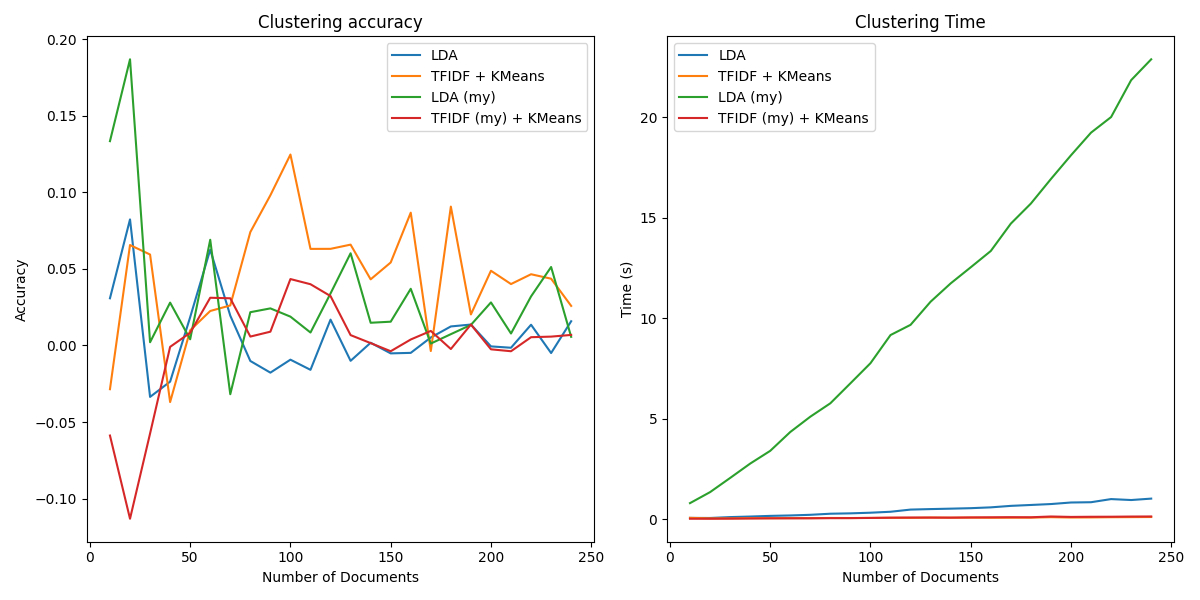
\includegraphics[width=\textwidth]{inc/res_250_2.png}
	\caption{Сравнение алгоритмов}
	\label{img:time4}
\end{figure}


Видно, что LDA (собственный и библиотечный) работают дольше TF-IDF + KMEANS. При этом точность кластеризации у всех алгоритмов относительно невысокая (до 0.2).


\chapter*{ЗАКЛЮЧЕНИЕ}
\addcontentsline{toc}{section}{ЗАКЛЮЧЕНИЕ}
В ходе выполнения работы были изучены TF-IDF и LDA.

Для достижения поставленной цели были решены задачи:
\begin{itemize}
	\item приведено описание алгоритмов;
	\item приведено описание используемых для исследования данных;
	\item приведены зависимости скорости и точности работы алгоритмов от объёма данных.
\end{itemize}

Проведенные исследования показали, что LDA (собственный и библиотечный) работают дольше TF-IDF + KMEANS. При этом точность кластеризации у всех алгоритмов относительно невысокая (до 0.2).

\pagebreak

\printbibliography[title={СПИСОК ИСПОЛЬЗОВАННЫХ\\ ИСТОЧНИКОВ}]
\addcontentsline{toc}{chapter}{СПИСОК ИСПОЛЬЗОВАННЫХ ИСТОЧНИКОВ}

\bibliographystyle{utf8gost705u}  % стилевой файл для оформления по ГОСТу       % имя библиографической базы (bib-файла) 

\pagebreak
\end{document}